\documentclass[12pt,a4paper]{report}
\usepackage[utf8]{inputenc}
\usepackage[T5]{fontenc}
\usepackage[vietnamese]{babel}
\usepackage{mathptmx} % Font tương đương Times New Roman trong LaTeX
\usepackage{amsmath,amsfonts,amssymb}
\usepackage{graphicx}
\usepackage{booktabs}
\usepackage{array}
\usepackage{longtable}
\usepackage{geometry}
\usepackage[hidelinks]{hyperref}
\usepackage{float}
\usepackage{caption}
\usepackage{setspace}
\usepackage{fancyhdr}
\usepackage{titlesec}
\usepackage{listings}
\usepackage{xcolor}
\usepackage{indentfirst}

% 1. Quy định lề trang: Trên 2.0cm, Dưới 2.0cm, Trái 2.5cm, Phải 2.0cm
\geometry{a4paper, top=2.0cm, bottom=2.0cm, left=2.5cm, right=2.0cm}

% 2. Quy định cỡ chữ 13pt và giãn dòng 1.5
\renewcommand{\normalsize}{\fontsize{13pt}{19.5pt}\selectfont}
\onehalfspacing

% 3. Quy định đánh số trang ở giữa, phía dưới; trang bìa không hiển thị
\pagestyle{fancy}
\fancyhf{}
\fancyfoot[C]{\fontsize{12pt}{14pt}\selectfont \thepage}
\renewcommand{\headrulewidth}{0pt}
\renewcommand{\footrulewidth}{0pt}

\fancypagestyle{plain}{
    \fancyhf{}
    \fancyfoot[C]{\fontsize{12pt}{14pt}\selectfont \thepage}
    \renewcommand{\headrulewidth}{0pt}
    \renewcommand{\footrulewidth}{0pt}
}

% 4. Quy định tên bảng trên bảng, tên hình dưới hình; căn giữa, in nghiêng, cỡ 12pt
\captionsetup{
    font={normalsize,it},
    labelfont={bf,it},
    justification=centering,
    labelsep=colon
}
\captionsetup[table]{position=top, skip=6pt}
\captionsetup[figure]{position=bottom, skip=6pt}

% Định dạng tiêu đề Chương và Mục thống nhất
\titleformat{\chapter}[display]
  {\normalfont\fontsize{16pt}{20pt}\bfseries\centering}
  {CHƯƠNG \thechapter}{10pt}{\fontsize{16pt}{20pt}\bfseries\MakeUppercase}
\titlespacing*{\chapter}{0pt}{-10pt}{20pt}

\titleformat{\section}
  {\normalfont\fontsize{14pt}{18pt}\bfseries}{\thesection}{1em}{}
\titleformat{\subsection}
  {\normalfont\fontsize{13pt}{17pt}\bfseries\itshape}{\thesubsection}{1em}{}

% Định dạng hiển thị mã nguồn trong Phụ lục
\lstset{
    basicstyle=\ttfamily\fontsize{10pt}{12pt}\selectfont,
    breaklines=true,
    frame=single,
    backgroundcolor=\color{gray!8},
    keywordstyle=\color{blue}\bfseries,
    commentstyle=\color{green!50!black}\itshape,
    stringstyle=\color{red!70!black},
    showstringspaces=false,
    numbers=left,
    numberstyle=\tiny\color{gray}
}

\begin{document}

% =========================================================================
% TRANG BÌA (Không đánh số trang)
% =========================================================================
\begin{titlepage}
    \thispagestyle{empty}
    \centering
    \textbf{\fontsize{14pt}{18pt}\selectfont TRƯỜNG ĐẠI HỌC ĐẠI NAM}\\
    \textbf{\fontsize{14pt}{18pt}\selectfont KHOA CÔNG NGHỆ THÔNG TIN}\\[2.2cm]
    
    \textbf{\fontsize{15pt}{20pt}\selectfont BÁO CÁO BÀI TẬP LỚN HỌC PHẦN}\\
    \textbf{\fontsize{16pt}{22pt}\selectfont NHẬP MÔN HỌC MÁY (FIT4013)}\\[1.2cm]
    
    \rule{\linewidth}{0.6mm}\\[0.5cm]
    {\fontsize{17pt}{24pt}\selectfont \textbf{ĐỀ TÀI 3: XÂY DỰNG HỆ THỐNG PHÂN LOẠI TIN NHẮN RÁC (SMS SPAM DETECTION) SỬ DỤNG CÁC THUẬT TOÁN HỌC MÁY}}\\[0.3cm]
    \rule{\linewidth}{0.6mm}\\[2.2cm]
    
    \begin{flushleft}
        \large
        \textbf{Giảng viên hướng dẫn:} ThS. Lê Thị Thùy Trang\\[0.3cm]
        \textbf{Nhóm thực hiện:} Nhóm 10\\[0.3cm]
        \textbf{Sinh viên thực hiện:} Đoàn Quốc Bảo, Hà Minh Quân\\[0.3cm]
        \textbf{Mã nguồn GitHub:} \url{https://github.com/dathu2006/FIT4013-SMS-Spam-Classification}
    \end{flushleft}
    
    \vfill
    {\fontsize{13pt}{18pt}\selectfont \textbf{Hà Nội, Năm 2026}}
\end{titlepage}

% Mục lục, Danh mục hình ảnh, Danh mục bảng biểu
\pagenumbering{roman}
\tableofcontents
\newpage
\listoffigures
\listoftables
\newpage

% Bắt đầu đánh số trang 1 cho nội dung chính
\pagenumbering{arabic}
\setcounter{page}{1}

% =========================================================================
% PHẦN MỞ ĐẦU
% =========================================================================
\chapter*{PHẦN MỞ ĐẦU}
\addcontentsline{toc}{chapter}{PHẦN MỞ ĐẦU}

\section*{1. Tính cấp thiết của đề tài}
Trong kỷ nguyên bùng nổ của viễn thông di động và các dịch vụ số, dịch vụ tin nhắn ngắn (Short Message Service -- SMS) vẫn giữ vai trò kênh giao tiếp cốt lõi nhờ tính phổ cập trên mọi thiết bị đầu cuối mà không phụ thuộc vào kết nối Internet. Tuy nhiên, song song với sự tiện lợi đó là sự gia tăng chóng mặt của vấn nạn tin nhắn rác (SMS Spam). Tin nhắn rác không chỉ dừng lại ở các thông điệp quảng cáo thương mại trái phép gây phiền nhiễu cho người dùng, mà còn biến tướng thành các chiến dịch lừa đảo tài chính tinh vi (Smishing -- SMS Phishing), giả mạo ngân hàng, thông báo trúng thưởng ảo hoặc phát tán đường dẫn chứa mã độc đánh cắp thông tin cá nhân.

Các phương pháp lọc truyền thống dựa trên danh sách đen số điện thoại (Blacklist) hoặc bộ lọc từ khóa cứng (Rule-based filtering) ngày càng bộc lộ nhiều hạn chế nghiêm trọng. Kẻ phát tán tin nhắn rác liên tục thay đổi đầu số gửi tin, sử dụng các từ viết tắt, chèn ký tự đặc biệt hoặc biến thể ngữ nghĩa để qua mặt các quy tắc tĩnh. Do đó, việc ứng dụng các kỹ thuật Học máy (Machine Learning) kết hợp Xử lý ngôn ngữ tự nhiên (Natural Language Processing -- NLP) để học tự động các đặc trưng thống kê và ngữ cảnh của tin nhắn, từ đó phân loại chính xác tin nhắn hợp lệ (\texttt{ham}) và tin nhắn rác (\texttt{spam}), là hướng tiếp cận thiết yếu và mang lại giá trị thực tiễn cao.

\section*{2. Mục tiêu nghiên cứu}
Bài tập lớn hướng tới các mục tiêu cụ thể sau:
\begin{itemize}
    \item Phân tích khám phá dữ liệu (EDA) trên bộ ngữ liệu chuẩn quốc tế \textit{SMS Spam Collection v.1} nhằm nhận diện các quy luật phân phối nhãn, cấu trúc độ dài văn bản và đặc trưng ký tự giữa hai lớp \texttt{ham} và \texttt{spam}.
    \item Xây dựng quy trình xử lý dữ liệu học máy chuẩn mực, đảm bảo tính tái tạo (reproducibility) và ngăn chặn triệt để hiện tượng rò rỉ dữ liệu (data leakage).
    \item Thiết kế phương pháp tiền xử lý văn bản chuyên biệt cho dữ liệu SMS thông qua việc chuẩn hóa các mẫu biểu thức chính quy thành các token ngữ nghĩa (\texttt{token\_url}, \texttt{token\_money}, \texttt{token\_num}, \texttt{token\_exclam}) kết hợp biểu diễn TF-IDF n-gram, đối chiếu trực tiếp với phương pháp Bag-of-Words cơ bản.
    \item Huấn luyện, tinh chỉnh tham số và so sánh định lượng hiệu năng của ba thuật toán học máy kinh điển: \textit{Multinomial Naive Bayes}, \textit{Decision Tree} và \textit{K-Nearest Neighbors}.
    \item Đóng gói mô hình tối ưu và xây dựng ứng dụng giao diện web tương tác bằng thư viện Streamlit phục vụ kiểm thử trực quan theo thời gian thực.
\end{itemize}

\section*{3. Đối tượng và phạm vi nghiên cứu}
\begin{itemize}
    \item \textbf{Đối tượng nghiên cứu:} Dữ liệu văn bản tin nhắn SMS tiếng Anh và các thuật toán học máy có giám sát (Supervised Learning) áp dụng cho bài toán phân loại văn bản nhị phân.
    \item \textbf{Phạm vi dữ liệu:} Bộ dữ liệu \textit{SMS Spam Collection v.1} gồm 5.572 mẫu tin nhắn thực tế được công bố bởi Tiago A. Almeida và José María Gómez Hidalgo.
    \item \textbf{Phạm vi công nghệ:} Ngôn ngữ lập trình Python 3.9 cùng hệ sinh thái thư viện khoa học dữ liệu (\texttt{pandas}, \texttt{numpy}, \texttt{scikit-learn}, \texttt{matplotlib}, \texttt{seaborn}, \texttt{joblib}) và khung phát triển ứng dụng web \texttt{Streamlit}.
\end{itemize}

\section*{4. Phương pháp nghiên cứu}
Đề tài kết hợp chặt chẽ giữa nghiên cứu lý thuyết và thực nghiệm định lượng:
\begin{itemize}
    \item \textbf{Phương pháp phân tích thống kê mô tả:} Sử dụng các đại lượng thống kê (trung bình, trung vị, tứ phân vị) và biểu đồ trực quan hóa để khám phá đặc điểm dữ liệu thô.
    \item \textbf{Phương pháp thực nghiệm đối chứng (Ablation \& Comparative Study):} Thiết lập mô hình cơ sở (Baseline) làm thước đo chuẩn, sau đó thay đổi có kiểm soát từng thành phần (kỹ thuật trích xuất đặc trưng, thuật toán phân loại, siêu tham số làm mượt) trên cùng một tập kiểm thử độc lập để đánh giá tác động thực sự của từng cải tiến.
    \item \textbf{Phương pháp phân tích lỗi định tính (Error Analysis):} Trích xuất các mẫu dự đoán sai (False Positives và False Negatives) để tìm hiểu nguyên nhân gốc rễ về mặt ngôn ngữ học và giới hạn của không gian đặc trưng.
\end{itemize}

\section*{5. Bố cục báo cáo}
Ngoài Phần mở đầu, Kết luận và Phụ lục, nội dung chính của báo cáo được tổ chức thành 3 chương:
\begin{itemize}
    \item \textbf{Chương 1 -- Cơ sở lý thuyết và Phân tích bài toán:} Trình bày tổng quan bài toán phân loại văn bản, phân tích khám phá dữ liệu chuyên sâu, cơ sở toán học của các kỹ thuật biểu diễn đặc trưng văn bản và ba thuật toán học máy sử dụng trong đề tài.
    \item \textbf{Chương 2 -- Thiết kế giải pháp và Triển khai hệ thống:} Mô tả kiến trúc tổng thể, quy trình làm sạch và chống rò rỉ dữ liệu, thiết kế hai luồng tiền xử lý đặc trưng, kịch bản thực nghiệm và cấu trúc mã nguồn ứng dụng web demo.
    \item \textbf{Chương 3 -- Thực nghiệm, Đánh giá kết quả và Thảo luận:} Trình bày kết quả định lượng của 7 kịch bản thí nghiệm, phân tích ma trận nhầm lẫn, đánh giá tầm quan trọng của đặc trưng qua chỉ số Log-odds và phân tích các trường hợp lỗi điển hình.
\end{itemize}

% =========================================================================
% CHƯƠNG 1: CƠ SỞ LÝ THUYẾT VÀ PHÂN TÍCH BÀI TOÁN
% =========================================================================
\chapter{CƠ SỞ LÝ THUYẾT VÀ PHÂN TÍCH BÀI TOÁN}

\section{Tổng quan bài toán phân loại tin nhắn rác}
\subsection{Phát biểu bài toán dưới góc độ Học máy}
Trong lĩnh vực Học máy, bài toán phân loại tin nhắn rác được mô hình hóa dưới dạng bài toán phân loại nhị phân có giám sát (Binary Supervised Classification). Cho tập dữ liệu huấn luyện gồm $N$ cặp mẫu:
\begin{equation}
    \mathcal{D} = \{(x_1, y_1), (x_2, y_2), \dots, (x_N, y_N)\}
\end{equation}
trong đó:
\begin{itemize}
    \item $x_i \in \mathcal{X}$ là chuỗi văn bản tin nhắn SMS thứ $i$ có độ dài biến thiên.
    \item $y_i \in \mathcal{Y} = \{0, 1\}$ là nhãn phân loại tương ứng, với $y_i = 0$ đại diện cho tin nhắn hợp lệ (\texttt{ham}) và $y_i = 1$ đại diện cho tin nhắn rác (\texttt{spam}).
\end{itemize}

Mục tiêu của quá trình học là tìm kiếm một ánh xạ tiền xử lý $\phi: \mathcal{X} \rightarrow \mathbb{R}^d$ để chuyển đổi văn bản phi cấu trúc thành vector đặc trưng số học $d$-chiều, đồng thời huấn luyện một hàm phân loại $f: \mathbb{R}^d \rightarrow \{0, 1\}$ sao cho cực tiểu hóa rủi ro kỳ vọng trên phân phối dữ liệu thực tế.

\subsection{Đặc thù chi phí sai lệch trong bài toán thực tế}
Khác với các bài toán phân loại thông thường có chi phí sai lệch đối xứng, hệ thống lọc tin nhắn rác có sự bất đối xứng rõ rệt về hậu quả của hai loại sai lầm:
\begin{itemize}
    \item \textbf{Dương tính giả (False Positive -- FP):} Hệ thống phân loại nhầm một tin nhắn hợp lệ (\texttt{ham}) thành tin nhắn rác (\texttt{spam}). Trong thực tế, việc chặn hoặc ẩn nhầm tin nhắn mã xác thực OTP ngân hàng, thông báo công việc hoặc tin nhắn từ người thân gây thiệt hại nghiêm trọng đến trải nghiệm và quyền lợi của người dùng.
    \item \textbf{Âm tính giả (False Negative -- FN):} Hệ thống bỏ sót một tin nhắn rác (\texttt{spam}) và phân loại thành tin nhắn hợp lệ (\texttt{ham}). Người dùng sẽ nhận tin nhắn quảng cáo trong hộp thư đến nhưng vẫn có thể tự nhận biết và xóa thủ công.
\end{itemize}

Do đó, bên cạnh độ chính xác tổng thể (\textit{Accuracy}), mô hình lọc SMS Spam bắt buộc phải ưu tiên tối ưu hóa chỉ số \textit{Precision} (tỷ lệ dự đoán spam chính xác) đạt mức rất cao, đồng thời duy trì chỉ số \textit{Recall} (tỷ lệ bắt được spam thực tế) ở mức tốt nhất có thể thông qua điểm cân bằng điều hòa $F_1$-score.

\section{Phân tích khám phá dữ liệu (EDA)}
\subsection{Nguồn gốc và cấu trúc bộ dữ liệu SMS Spam Collection}
Nghiên cứu sử dụng bộ dữ liệu \textbf{SMS Spam Collection v.1} do Tiago A. Almeida và José María Gómez Hidalgo xây dựng và công bố tại hội nghị quốc tế ACM Symposium on Document Engineering (DOCENG'11). Dữ liệu được tổng hợp từ bốn nguồn thực tế:
\begin{enumerate}
    \item Tập hợp 425 tin nhắn rác được trích xuất thủ công từ trang web báo cáo tin nhắn rác công cộng Grumbletext của Vương quốc Anh.
    \item Tập con gồm 3.375 tin nhắn hợp lệ được chọn ngẫu nhiên từ kho ngữ liệu NUS SMS Corpus (National University of Singapore).
    \item Tập hợp 450 tin nhắn hợp lệ thu thập từ luận án tiến sĩ của Caroline Tag.
    \item Kho ngữ liệu SMS Spam Corpus v.0.1 Big gồm 1.002 tin nhắn hợp lệ và 322 tin nhắn rác.
\end{enumerate}

Dữ liệu thô lưu trữ trong tệp văn bản \texttt{SMSSpamCollection} theo định dạng phân tách bằng ký tự Tab (\texttt{TSV}), mỗi dòng gồm hai cột: cột nhãn (\texttt{ham} hoặc \texttt{spam}) và cột nội dung văn bản gốc.

\subsection{Thống kê phân phối lớp và tính toàn vẹn dữ liệu}
Tiến hành kiểm tra toàn diện trên 5.572 bản ghi của tập dữ liệu gốc, nhóm thu được các chỉ số thống kê tổng hợp như trình bày trong Bảng~\ref{tab:eda_stats}.

\begin{table}[H]
    \centering
    \caption{Thống kê mô tả các đặc trưng cơ bản của bộ dữ liệu SMS Spam Collection}
    \label{tab:eda_stats}
    \begin{tabular}{lccc}
        \toprule
        \textbf{Chỉ số thống kê} & \textbf{Toàn bộ dữ liệu} & \textbf{Lớp Ham (0)} & \textbf{Lớp Spam (1)} \\
        \midrule
        Số lượng mẫu ban đầu & 5.572 & 4.825 (86,59\%) & 747 (13,41\%) \\
        Số lượng giá trị khuyết thiếu (Null) & 0 & 0 & 0 \\
        Số bản ghi trùng lặp hoàn toàn & 403 (7,23\%) & 309 & 94 \\
        Số mẫu duy nhất sau làm sạch & 5.169 & 4.516 (87,37\%) & 653 (12,63\%) \\
        Độ dài trung bình (ký tự) & 80,49 & 71,48 & 138,67 \\
        Độ dài trung vị (ký tự) & 62,00 & 52,00 & 149,00 \\
        Số chữ số trung bình / tin nhắn & 2,38 & 0,30 & 15,81 \\
        Số chữ số trung vị / tin nhắn & 0,00 & 0,00 & 16,00 \\
        \bottomrule
    \end{tabular}
\end{table}

Từ số liệu Bảng~\ref{tab:eda_stats} và biểu đồ trực quan hóa ở Hình~\ref{fig:eda}, ba phát hiện quan trọng được rút ra để định hướng thiết kế đặc trưng:
\begin{itemize}
    \item \textbf{Hiện tượng mất cân bằng lớp (Class Imbalance):} Tin nhắn \texttt{ham} chiếm tới 86,59\% trong khi \texttt{spam} chỉ chiếm 13,41\% (tỷ lệ chênh lệch xấp xỉ $6,5 : 1$). Nếu một mô hình ngây thơ luôn dự đoán mọi tin nhắn là \texttt{ham}, độ chính xác \textit{Accuracy} vẫn đạt 86,59\% nhưng hoàn toàn vô dụng. Điều này khẳng định việc phân tầng dữ liệu (\textit{Stratified Split}) và đánh giá bằng $F_1$-score là bắt buộc.
    \item \textbf{Sự tồn tại của dữ liệu trùng lặp:} Có 403 tin nhắn lặp lại hoàn toàn nội dung (chiếm 7,23\%, đặc biệt tỷ lệ lặp ở lớp \texttt{spam} lên tới $94/747 = 12,58\%$ do tin nhắn quảng cáo thường được phát tán hàng loạt). Nếu không loại bỏ trước khi chia tập huấn luyện/kiểm thử, cùng một tin nhắn sẽ xuất hiện ở cả hai tập gây sai lệch kết quả đánh giá.
    \item \textbf{Quy luật phân bố độ dài và mật độ chữ số:} Tin nhắn \texttt{ham} thường ngắn gọn (trung vị 52 ký tự) và hầu như không chứa chữ số (trung vị bằng 0). Ngược lại, tin nhắn \texttt{spam} có độ dài tập trung sát giới hạn chuẩn 160 ký tự của một bản tin SMS (trung vị 149 ký tự) và chứa lượng chữ số vượt trội (trung vị 16 chữ số/tin nhắn) dùng để biểu thị số điện thoại tổng đài, mã nhận thưởng, giá trị tiền tệ hoặc thời hạn khuyến mãi.
\end{itemize}

\begin{figure}[H]
    \centering
    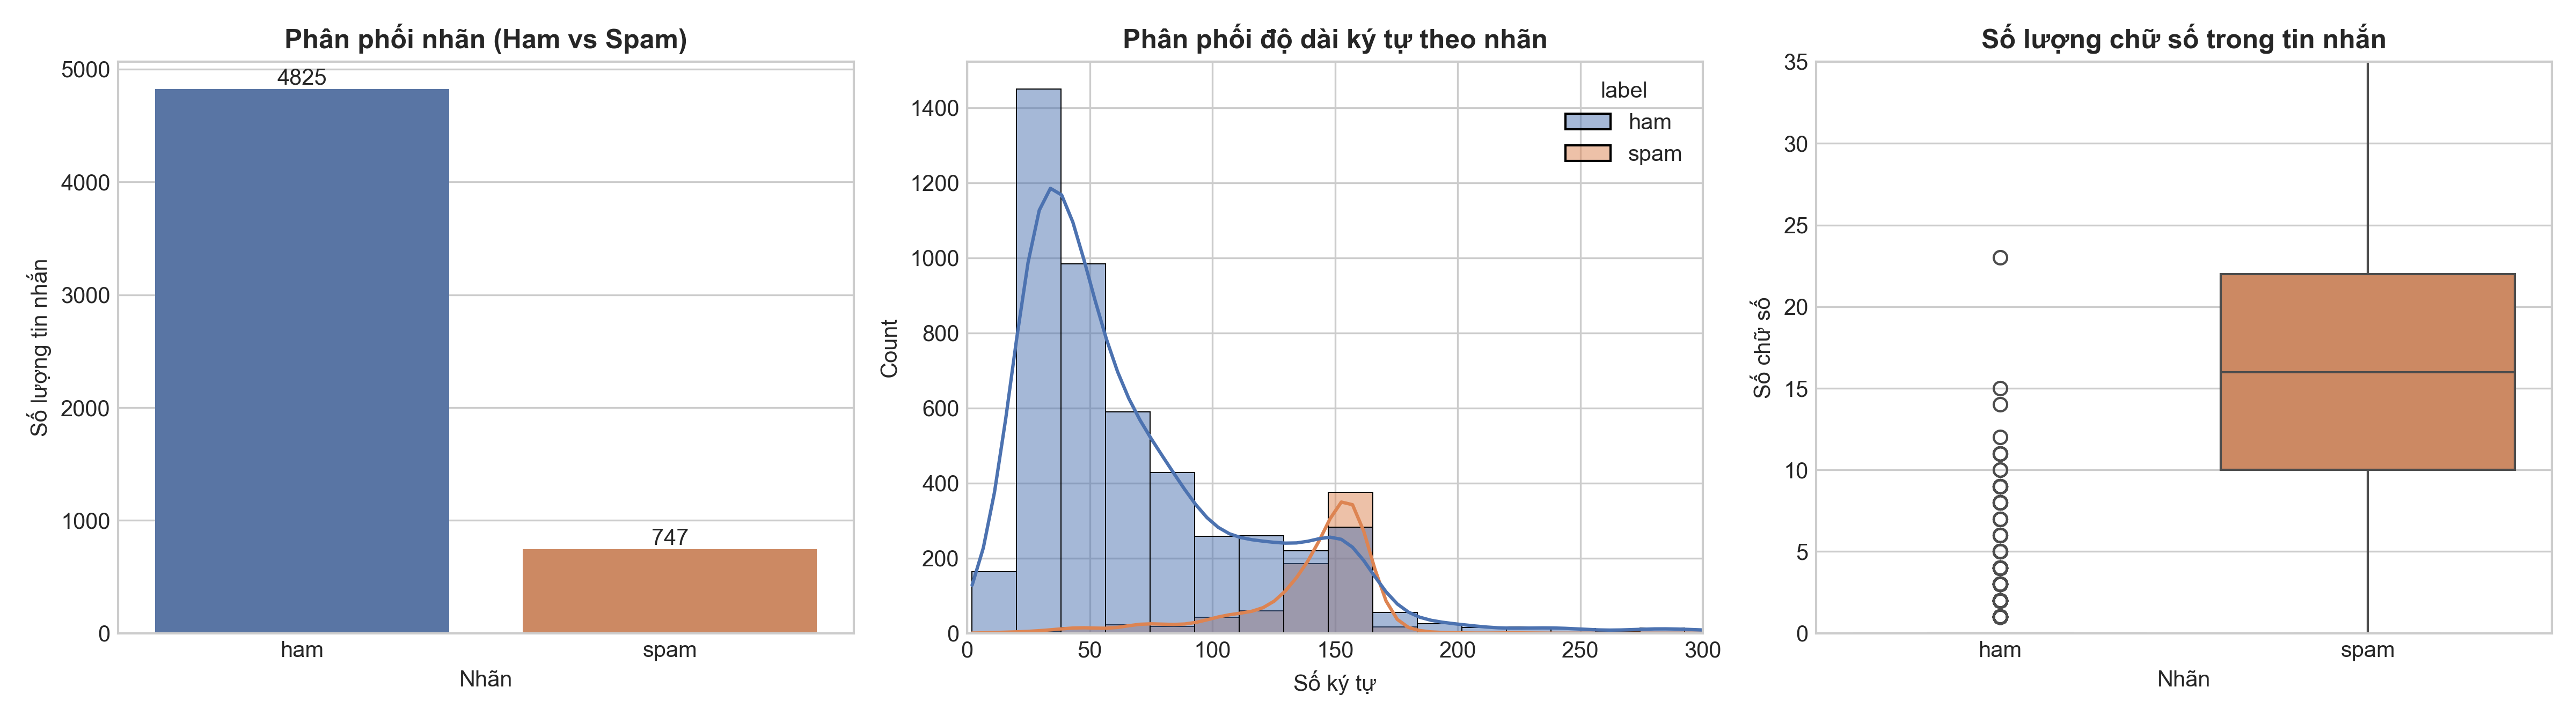
\includegraphics[width=\textwidth]{figures/eda_overview.png}
    \caption{Trực quan hóa phân phối nhãn, độ dài ký tự và số lượng chữ số theo từng lớp dữ liệu.}
    \label{fig:eda}
\end{figure}

\section{Cơ sở toán học của biểu diễn đặc trưng văn bản}
Các thuật toán học máy không thể xử lý trực tiếp chuỗi ký tự thô mà yêu cầu đầu vào là các vector số thực trong không gian Euclid. Giả sử sau quá trình tiền xử lý, kho ngữ liệu huấn luyện thu được bộ từ vựng $V = \{t_1, t_2, \dots, t_{|V|}\}$ gồm $|V|$ thuật ngữ (term) duy nhất.

\subsection{Mô hình túi từ (Bag-of-Words -- BoW)}
Mô hình Bag-of-Words biểu diễn mỗi văn bản $d$ thành một vector tần suất $v_d \in \mathbb{R}^{|V|}$, trong đó thành phần thứ $j$ được tính bằng số lần xuất hiện thô (term frequency) của thuật ngữ $t_j$ trong văn bản $d$:
\begin{equation}
    v_{d, j} = \text{tf}(t_j, d) = \sum_{w \in d} \mathbb{I}(w = t_j)
\end{equation}
Ưu điểm của BoW là đơn giản, bảo toàn thông tin tần suất xuất hiện tuyệt đối của từ khóa. Tuy nhiên, hạn chế cố hữu của BoW là đánh đồng vai trò của các từ phổ biến xuất hiện ở hầu hết các văn bản với các từ khóa đặc trưng mang tính phân loại cao, đồng thời làm mất hoàn toàn trật tự cú pháp cục bộ nếu chỉ xét từ đơn (unigram).

\subsection{Trọng số TF-IDF và mô hình N-gram}
Để khắc phục nhược điểm của BoW, phương pháp \textbf{TF-IDF} (Term Frequency -- Inverse Document Frequency) kết hợp tần suất xuất hiện cục bộ trong từng tin nhắn với độ hiếm của thuật ngữ trên toàn bộ tập huấn luyện $D$:
\begin{equation}
    \text{tfidf}(t, d, D) = \text{tf}(t, d) \times \text{idf}(t, D)
\end{equation}
Trong thư viện \texttt{scikit-learn}, thành phần nghịch đảo tần suất văn bản có làm mượt ($\text{smooth\_idf=True}$) được tính theo công thức:
\begin{equation}
    \text{idf}(t, D) = \ln \left( \frac{1 + |D|}{1 + \text{df}(t, D)} \right) + 1
\end{equation}
trong đó $|D|$ là tổng số văn bản huấn luyện và $\text{df}(t, D)$ là số lượng văn bản có chứa thuật ngữ $t$. Sau đó, mỗi vector đặc trưng của văn bản $d$ được chuẩn hóa theo chuẩn Euclid $L_2$ nhằm loại bỏ ảnh hưởng của độ dài tin nhắn:
\begin{equation}
    \hat{v}_d = \frac{v_d}{\|v_d\|_2} = \frac{v_d}{\sqrt{\sum_{j=1}^{|V|} v_{d,j}^2}}
\end{equation}

Bên cạnh đó, việc mở rộng không gian từ vựng sang \textbf{Bigram} ($n=2$) cho phép nắm bắt các cụm từ hai từ liền kề có ý nghĩa phân biệt mạnh như \textit{``have won''}, \textit{``your mobile''}, \textit{``to claim''}, vốn bị tách rời hoàn toàn trong mô hình Unigram truyền thống.

\section{Các thuật toán Học máy sử dụng trong đề tài}
\subsection{Multinomial Naive Bayes (MNB)}
Multinomial Naive Bayes là biến thể của họ thuật toán phân loại xác suất dựa trên Định lý Bayes, được thiết kế chuyên biệt cho dữ liệu rời rạc và ma trận tần suất văn bản. Với một tin nhắn được biểu diễn bởi vector đặc trưng $x = (x_1, x_2, \dots, x_{|V|})$, xác suất hậu nghiệm để $x$ thuộc lớp $c \in \{0, 1\}$ được tính theo công thức:
\begin{equation}
    P(y = c \mid x) = \frac{P(y = c) \prod_{j=1}^{|V|} P(t_j \mid y = c)^{x_j}}{P(x)}
\end{equation}

Nhờ giả định độc lập có điều kiện giữa các đặc trưng khi biết trước nhãn lớp, quy tắc quyết định tối ưu (Maximum A Posteriori -- MAP) trong không gian logarit trở thành hàm tuyến tính:
\begin{equation}
    \hat{y} = \arg\max_{c \in \{0, 1\}} \left[ \log P(y = c) + \sum_{j=1}^{|V|} x_j \log P(t_j \mid y = c) \right]
\end{equation}

Để tránh hiện tượng xác suất bằng $0$ khi gặp từ vựng mới chưa từng xuất hiện trong lớp $c$ ở tập huấn luyện, ước lượng hợp lý cực đại được hiệu chỉnh bằng kỹ thuật \textbf{làm mượt Laplace/Lidstone} với siêu tham số $\alpha > 0$:
\begin{equation}
    \hat{\theta}_{c, j} = P(t_j \mid y = c) = \frac{N_{c, j} + \alpha}{N_c + \alpha |V|}
\end{equation}
trong đó $N_{c, j} = \sum_{x_i \in D_c} x_{i, j}$ là tổng trọng số của thuật ngữ $t_j$ trong toàn bộ văn bản thuộc lớp $c$, và $N_c = \sum_{j=1}^{|V|} N_{c, j}$ là tổng trọng số của mọi thuật ngữ trong lớp $c$. Khi $\alpha = 1.0$, phép ước lượng gọi là làm mượt Laplace; khi $0 < \alpha < 1$, gọi là làm mượt Lidstone, giúp giảm bớt sự chi phối của phân phối đều lên các lớp thiểu số.

\subsection{Decision Tree (Cây quyết định)}
Thuật toán Cây quyết định (CART) phân chia đệ quy không gian đặc trưng $d$-chiều thành các vùng không giao nhau dựa trên ngưỡng giá trị của từng đặc trưng đơn lẻ. Tại mỗi nút trong $m$, thuật toán tìm kiếm cặp đặc trưng $j$ và ngưỡng $s$ sao cho cực tiểu hóa độ bất thuần khiết (Impurity) của hai nút con trái và phải. Với độ đo Gini Impurity, hàm mục tiêu tại nút $m$ được xác định bởi:
\begin{equation}
    G(m) = \sum_{c \in \{0, 1\}} p_{m, c}(1 - p_{m, c}) = 1 - \sum_{c \in \{0, 1\}} p_{m, c}^2
\end{equation}
trong đó $p_{m, c}$ là tỷ lệ mẫu thuộc lớp $c$ tại nút $m$. Trong dữ liệu văn bản có số chiều lớn (hàng nghìn từ vựng), cây quyết định dễ bị quá khớp (overfitting) nếu phát triển tự do; do đó tham số chiều sâu tối đa (\texttt{max\_depth}) đóng vai trò điều chuẩn quan trọng.

\subsection{K-Nearest Neighbors (K-NN)}
K-Nearest Neighbors là thuật toán học lười (lazy learning) không xây dựng hàm tham số tường minh trong pha huấn luyện mà lưu trữ toàn bộ tập mẫu đã chuẩn hóa. Khi dự đoán một tin nhắn mới $x$, thuật toán tìm tập $\mathcal{N}_k(x)$ gồm $k$ mẫu huấn luyện gần $x$ nhất và quyết định nhãn theo nguyên tắc bỏ phiếu đa số.

Đối với dữ liệu văn bản thưa chiều cao, khoảng cách Euclid truyền thống thường kém hiệu quả do bị chi phối bởi độ dài văn bản. Thay vào đó, \textbf{khoảng cách Cosine} được ưu tiên sử dụng để đo lường sự sai khác về góc hướng giữa hai vector đặc trưng $u$ và $v$:
\begin{equation}
    d_{\text{cosine}}(u, v) = 1 - \frac{u \cdot v}{\|u\|_2 \|v\|_2} = 1 - \frac{\sum_{j=1}^{|V|} u_j v_j}{\sqrt{\sum_{j=1}^{|V|} u_j^2}\sqrt{\sum_{j=1}^{|V|} v_j^2}}
\end{equation}
Giá trị $d_{\text{cosine}} \in [0, 1]$ đạt cực tiểu bằng $0$ khi hai tin nhắn có tỷ lệ phân bố từ vựng hoàn toàn tương đồng.

\section{Các chỉ số đánh giá hiệu năng mô hình}
Từ ma trận nhầm lẫn (Confusion Matrix) gồm bốn thành phần $TP$ (True Positive), $TN$ (True Negative), $FP$ (False Positive) và $FN$ (False Negative) với lớp dương tính là \texttt{spam}, bốn độ đo chuẩn được sử dụng để đánh giá toàn diện mô hình:
\begin{align}
    \text{Accuracy} &= \frac{TP + TN}{TP + TN + FP + FN} \\
    \text{Precision} &= \frac{TP}{TP + FP} \\
    \text{Recall} &= \frac{TP}{TP + FN} \\
    F_1\text{-score} &= 2 \cdot \frac{\text{Precision} \times \text{Recall}}{\text{Precision} + \text{Recall}} = \frac{2TP}{2TP + FP + FN}
\end{align}

% =========================================================================
% CHƯƠNG 2: THIẾT KẾ GIẢI PHÁP VÀ TRIỂN KHAI HỆ THỐNG
% =========================================================================
\chapter{THIẾT KẾ GIẢI PHÁP VÀ TRIỂN KHAI HỆ THỐNG}

\section{Kiến trúc quy trình học máy và kiểm soát rò rỉ dữ liệu}
Để đảm bảo tính khách quan khoa học và khả năng tái tạo kết quả trên mọi môi trường thực thi, hệ thống được thiết kế theo đường ống (pipeline) khép kín gồm 6 giai đoạn tuần tự:
\begin{center}
    \textbf{Dữ liệu thô} $\rightarrow$ \textbf{Khử trùng lặp} $\rightarrow$ \textbf{Phân tầng Train/Test} $\rightarrow$ \textbf{Tiền xử lý} $\rightarrow$ \textbf{Vector hóa} $\rightarrow$ \textbf{Huấn luyện \& Đánh giá}
\end{center}

Một sai lầm phổ biến trong các bài toán xử lý văn bản là thực hiện trích xuất từ vựng (\texttt{fit}) trên toàn bộ tập dữ liệu trước khi chia tách Train/Test, dẫn đến hiện tượng \textit{rò rỉ dữ liệu} (data leakage) khi mô hình vô tình biết trước phân phối từ vựng của tập kiểm thử. Hệ thống áp dụng ba nguyên tắc kiểm soát nghiêm ngặt:
\begin{enumerate}
    \item \textbf{Loại bỏ trùng lặp trước khi phân chia:} Toàn bộ 403 dòng trùng lặp trong 5.572 bản ghi gốc được lọc bỏ ngay ở bước đầu tiên, giữ lại chính xác \textbf{5.169} tin nhắn độc nhất (4.516 \texttt{ham} và 653 \texttt{spam}).
    \item \textbf{Phân chia phân tầng cố định hạt giống ngẫu nhiên:} Tập dữ liệu sạch được chia theo tỷ lệ \textbf{80\% huấn luyện} (4.135 mẫu: 3.613 \texttt{ham}, 522 \texttt{spam}) và \textbf{20\% kiểm thử} (1.034 mẫu: 903 \texttt{ham}, 131 \texttt{spam}) với tham số \texttt{stratify=y} và \texttt{random\_state=42} nhằm bảo toàn nguyên vẹn tỷ lệ mất cân bằng lớp 87,37\% / 12,63\% trên cả hai tập.
    \item \textbf{Cô lập bộ biến đổi đặc trưng:} Các đối tượng \texttt{CountVectorizer} và \texttt{TfidfVectorizer} chỉ được phép học từ vựng và tính trọng số IDF duy nhất trên tập huấn luyện thông qua hàm \texttt{fit\_transform(X\_train)}. Tập kiểm thử chỉ đi qua phép chiếu \texttt{transform(X\_test)}.
\end{enumerate}

\section{Thiết kế hai phương án tiền xử lý và trích xuất đặc trưng}
Nhằm kiểm chứng giả thuyết khoa học rằng việc bảo tồn cấu trúc chữ số, tiền tệ và dấu câu đặc thù của tin nhắn SMS sẽ giúp cải thiện đáng kể khả năng nhận diện tin nhắn rác, nhóm thiết kế song song hai luồng tiền xử lý độc lập.

\subsection{Phương án 1: Tiền xử lý cơ bản (Baseline Pipeline)}
Phương án này tuân theo quy trình làm sạch văn bản truyền thống trong NLP:
\begin{itemize}
    \item Chuyển đổi toàn bộ ký tự về dạng chữ thường (\texttt{lowercase}).
    \item Sử dụng biểu thức chính quy \texttt{[\^{}a-z\textbackslash s]} để xóa bỏ hoàn toàn mọi chữ số, ký hiệu tiền tệ, dấu chấm câu và ký tự đặc biệt.
    \item Chuẩn hóa các khoảng trắng thừa về một dấu cách đơn.
    \item Biểu diễn bằng \texttt{CountVectorizer} ở mức từ đơn (\texttt{ngram\_range=(1,1)}), thu được ma trận thưa kích thước $4.135 \times 6.862$.
\end{itemize}

\subsection{Phương án 2: Tiền xử lý nâng cao chuyên biệt cho SMS (Enhanced Pipeline)}
Xuất phát từ phát hiện trong giai đoạn EDA rằng tin nhắn \texttt{spam} chứa mật độ chữ số (số điện thoại, mã thưởng) và ký hiệu tiền tệ vượt trội so với \texttt{ham}, việc xóa bỏ chúng như ở Phương án 1 sẽ làm mất đi những tín hiệu phân loại đắt giá nhất. Thay vì xóa bỏ, Phương án 2 thực hiện ánh xạ ngữ nghĩa bằng chuỗi biểu thức chính quy theo thứ tự ưu tiên được trình bày trong Bảng~\ref{tab:regex_rules}.

\begin{table}[H]
    \centering
    \caption{Quy tắc chuẩn hóa biểu thức chính quy thành Token ngữ nghĩa trong Phương án 2}
    \label{tab:regex_rules}
    \begin{tabular}{clp{6.2cm}}
        \toprule
        \textbf{Thứ tự} & \textbf{Biểu thức chính quy (Regex)} & \textbf{Token thay thế và ý nghĩa ngữ cảnh} \\
        \midrule
        1 & \texttt{https?://\textbackslash S+|www\textbackslash.\textbackslash S+} & Thay bằng \texttt{token\_url}: Nhận diện liên kết quảng cáo, trang nhận thưởng hoặc lừa đảo. \\
        2 & \texttt{[\pounds\$\textbackslash u20ac]\textbackslash s*\textbackslash d+|\textbackslash d+\textbackslash s*(gbp|usd|vnd)} & Thay bằng \texttt{token\_money}: Nhận diện giá trị giải thưởng, cước phí tin nhắn hoặc tiền mặt. \\
        3 & \texttt{\textbackslash b\textbackslash d+\textbackslash b|\textbackslash d+} & Thay bằng \texttt{token\_num}: Chuẩn hóa mọi số điện thoại tổng đài, mã code, thời hạn về một đặc trưng thống nhất. \\
        4 & \texttt{!+} & Thay bằng \texttt{token\_exclam}: Nắm bắt sắc thái cảm xúc khẩn cấp, kêu gọi hành động thường gặp trong spam. \\
        5 & \texttt{[\^{}a-z\_\textbackslash s]} & Loại bỏ các dấu câu nhiễu còn lại nhưng bảo toàn dấu gạch dưới của các token mới tạo. \\
        \bottomrule
    \end{tabular}
\end{table}

Sau bước chuẩn hóa token, văn bản được vector hóa bằng \texttt{TfidfVectorizer} với các cấu hình tinh chỉnh:
\begin{itemize}
    \item \textbf{Kết hợp từ đơn và cụm từ đôi (\texttt{ngram\_range=(1, 2)}):} Giúp mô hình học được các cấu trúc cụm từ đặc trưng như \texttt{call token\_num}, \texttt{token\_money prize}, \texttt{urgent token\_exclam}.
    \item \textbf{Lọc nhiễu tần suất (\texttt{min\_df=2, max\_df=0.95}):} Loại bỏ các từ sai chính tả chỉ xuất hiện duy nhất 1 lần trong toàn bộ tập huấn luyện nhằm giảm chiều không gian và chống quá khớp, đồng thời loại bỏ các từ quá phổ biến xuất hiện trên 95\% số tin nhắn.
\end{itemize}
Kết quả thu được ma trận đặc trưng TF-IDF có kích thước $4.135 \times 10.167$.

\section{Thiết kế kịch bản thực nghiệm so sánh}
Để đánh giá toàn diện cả yếu tố trích xuất đặc trưng lẫn thuật toán học máy, nhóm thiết kế 7 kịch bản thí nghiệm trên cùng tập dữ liệu kiểm thử gồm 1.034 mẫu (Bảng~\ref{tab:exp_setup}).

\begin{table}[H]
    \centering
    \caption{Danh mục 7 kịch bản thí nghiệm đối chứng}
    \label{tab:exp_setup}
    \begin{tabular}{clll}
        \toprule
        \textbf{Mã TN} & \textbf{Thuật toán phân loại} & \textbf{Biểu diễn đặc trưng} & \textbf{Siêu tham số chính} \\
        \midrule
        TN 1 & Multinomial Naive Bayes & BoW cơ bản (Unigram) & $\alpha = 1.0$ (\textbf{Baseline}) \\
        TN 2 & Decision Tree & BoW cơ bản (Unigram) & \texttt{max\_depth=20, random\_state=42} \\
        TN 3 & K-Nearest Neighbors & BoW cơ bản (Unigram) & \texttt{n\_neighbors=5, metric='cosine'} \\
        TN 4 & Multinomial Naive Bayes & TF-IDF cải tiến (1,2-gram) & $\alpha = 1.0$ \\
        TN 5 & Multinomial Naive Bayes & TF-IDF cải tiến (1,2-gram) & $\alpha = 0.2$ (Tinh chỉnh Lidstone) \\
        TN 6 & Decision Tree & TF-IDF cải tiến (1,2-gram) & \texttt{max\_depth=20, random\_state=42} \\
        TN 7 & K-Nearest Neighbors & TF-IDF cải tiến (1,2-gram) & \texttt{n\_neighbors=5, metric='cosine'} \\
        \bottomrule
    \end{tabular}
\end{table}

\section{Tổ chức mã nguồn và ứng dụng Web Demo}
Toàn bộ dự án được tổ chức theo cấu trúc thư mục tiêu chuẩn hóa của khoa học dữ liệu và quản lý phiên bản bằng Git/GitHub:
\begin{itemize}
    \item \texttt{data/SMSSpamCollection}: Kho dữ liệu gốc đầu vào.
    \item \texttt{notebooks/01\_eda\_and\_modeling.ipynb}: Sổ tay thực nghiệm tích hợp đầy đủ mã nguồn phân tích EDA, tiền xử lý, huấn luyện 7 kịch bản, trích xuất biểu đồ và xuất tệp mô hình.
    \item \texttt{models/}: Thư mục lưu trữ hai đối tượng đã huấn luyện gồm \texttt{tfidf\_vectorizer.joblib} và \texttt{mnb\_spam\_classifier.joblib}.
    \item \texttt{reports/figures/}: Lưu trữ các biểu đồ phân tích chất lượng cao (300 DPI) phục vụ báo cáo.
    \item \texttt{app.py}: Ứng dụng web tương tác xây dựng bằng thư viện \textbf{Streamlit}. Ứng dụng nạp trực tiếp hai tệp \texttt{.joblib} từ thư mục \texttt{models/}, áp dụng chính xác hàm tiền xử lý nâng cao lên tin nhắn người dùng nhập vào, hiển thị nhãn dự đoán (\texttt{HAM} hoặc \texttt{SPAM}) kèm thanh đo xác suất tin cậy $P(y=1 \mid x)$ theo thời gian thực, đồng thời hỗ trợ quản lý phiên đăng nhập và lưu trữ lịch sử kiểm tra tin nhắn.
\end{itemize}

\begin{figure}[H]
    \centering
    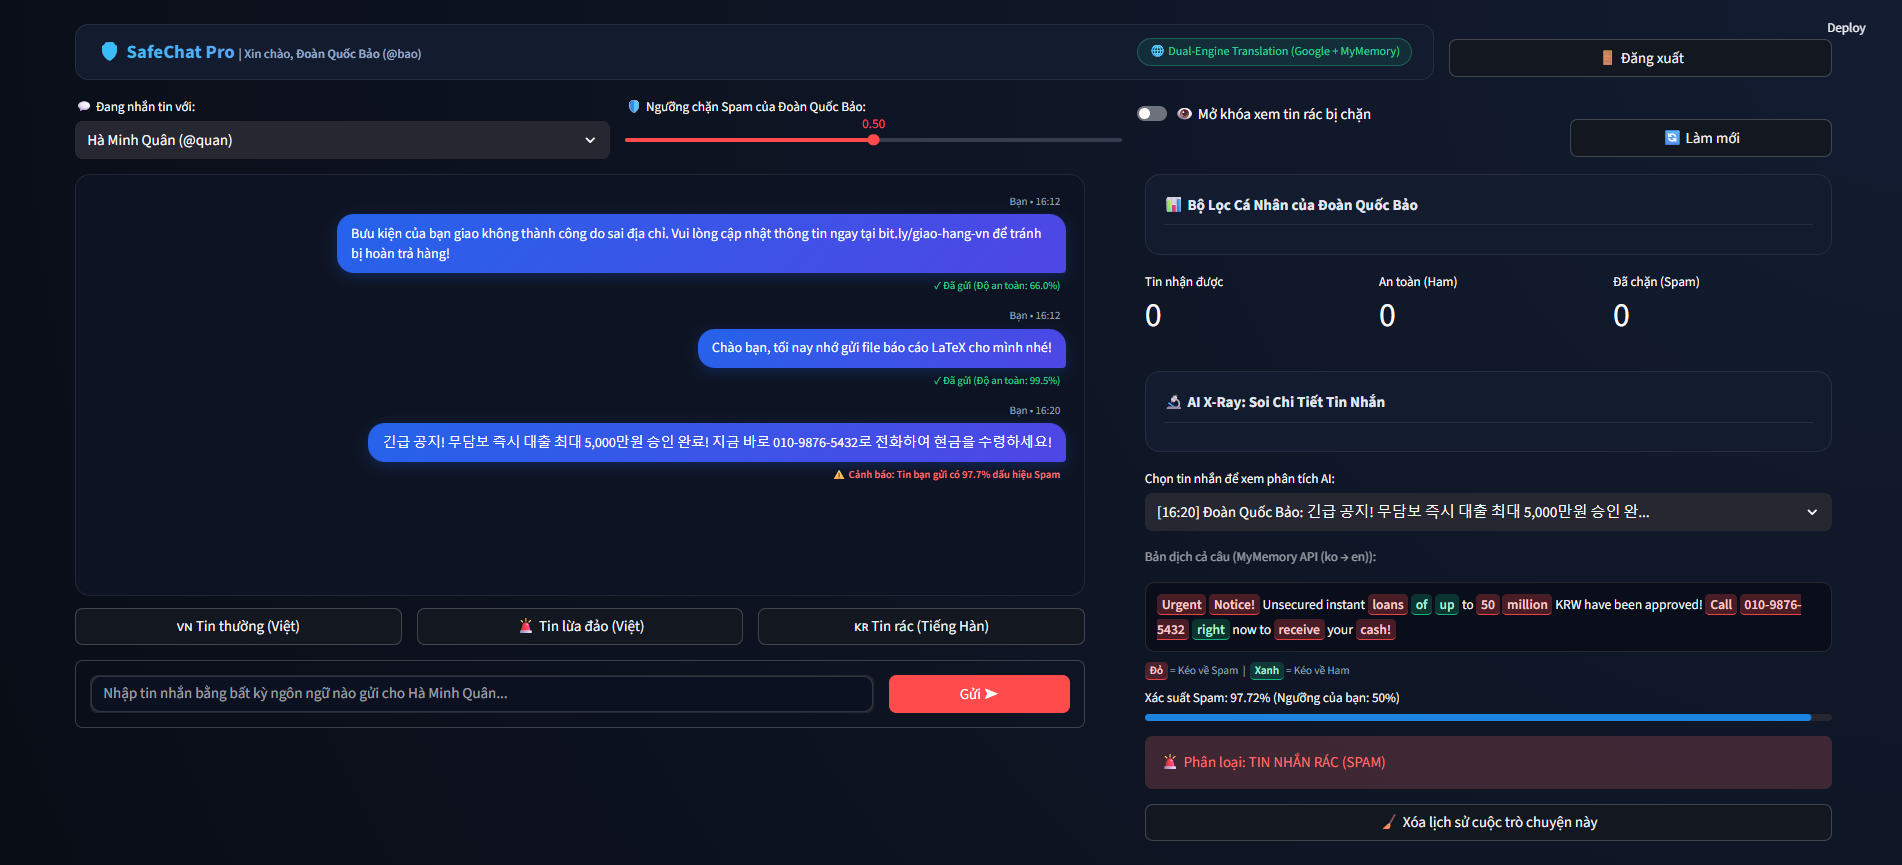
\includegraphics[width=0.92\textwidth]{figures/demo_app.png}
    \caption{Giao diện ứng dụng Web Demo phân loại tin nhắn rác theo thời gian thực xây dựng bằng Streamlit.}
    \label{fig:demo}
\end{figure}

% =========================================================================
% CHƯƠNG 3: THỰC NGHIỆM, ĐÁNH GIÁ KẾT QUẢ VÀ THẢO LUẬN
% =========================================================================
\chapter{THỰC NGHIỆM, ĐÁNH GIÁ KẾT QUẢ VÀ THẢO LUẬN}

\section{Kết quả định lượng trên tập kiểm thử độc lập}
Sau khi huấn luyện trên 4.135 mẫu và đánh giá trên 1.034 mẫu của tập kiểm thử độc lập (gồm 903 \texttt{ham} và 131 \texttt{spam}), kết quả chi tiết của 7 kịch bản thí nghiệm được tổng hợp trong Bảng~\ref{tab:results}.

\begin{table}[H]
    \centering
    \caption{Bảng tổng hợp kết quả thực nghiệm của 7 phương án trên tập kiểm thử (1.034 mẫu)}
    \label{tab:results}
    \resizebox{\textwidth}{!}{%
    \begin{tabular}{lccccc}
        \toprule
        \textbf{Kịch bản thí nghiệm} & \textbf{Accuracy (\%)} & \textbf{Precision (\%)} & \textbf{Recall (\%)} & \textbf{F1-score (\%)} & \textbf{Train (s)} \\
        \midrule
        1. [Baseline] MNB ($\alpha=1.0$) + BoW cơ bản & 98,07 & 93,70 & 90,84 & 92,25 & 0,0034 \\
        2. Decision Tree ($\text{depth}=20$) + BoW cơ bản & 96,71 & 90,08 & 83,21 & 86,51 & 0,0733 \\
        3. K-NN ($k=5$, cosine) + BoW cơ bản & 97,00 & 95,45 & 80,15 & 87,14 & 0,0020 \\
        \midrule
        4. MNB ($\alpha=1.0$) + TF-IDF cải tiến & 97,39 & \textbf{100,00} & 79,39 & 88,51 & 0,0030 \\
        \textbf{5. MNB ($\alpha=0.2$) + TF-IDF cải tiến} & \textbf{98,84} & \textbf{100,00} & \textbf{90,84} & \textbf{95,20} & 0,0040 \\
        6. Decision Tree ($\text{depth}=20$) + TF-IDF cải tiến & 97,49 & 92,68 & 87,02 & 89,76 & 0,2064 \\
        7. K-NN ($k=5$, cosine) + TF-IDF cải tiến & 97,10 & 98,10 & 78,63 & 87,29 & 0,0020 \\
        \bottomrule
    \end{tabular}%
    }
\end{table}

Từ số liệu Bảng~\ref{tab:results}, kịch bản \textbf{Thí nghiệm 5 (Multinomial Naive Bayes với $\alpha=0.2$ kết hợp TF-IDF cải tiến)} đạt hiệu năng vượt trội trên tất cả các chỉ số đánh giá:
\begin{itemize}
    \item Độ chính xác tổng thể (\textit{Accuracy}) đạt \textbf{98,84\%} (dự đoán đúng $1.022 / 1.034$ tin nhắn), tăng $+0,77\%$ so với mốc Baseline.
    \item Độ chính xác lớp rác (\textit{Precision}) đạt tuyệt đối \textbf{100,00\%} ($119 / 119$ dự đoán spam đều chính xác), tăng mạnh $+6,30\%$ so với mốc Baseline (93,70\%).
    \item Chỉ số tổng hợp \textit{$F_1$-score} đạt \textbf{95,20\%}, vượt $+2,95\%$ so với mốc Baseline (92,25\%) và bỏ xa các mô hình Decision Tree (89,76\%) cũng như K-NN (87,29\%).
    \item Thời gian huấn luyện chỉ mất \textbf{0,0040 giây} (4 mili-giây), đáp ứng hoàn hảo yêu cầu triển khai hệ thống thời gian thực.
\end{itemize}

\section{Phân tích ma trận nhầm lẫn và trọng số đặc trưng}
\subsection{Đối chiếu ma trận nhầm lẫn giữa Baseline và Mô hình tối ưu}
Hình~\ref{fig:cm} trực quan hóa chi tiết sự phân bố dự đoán đúng và sai của mô hình Baseline (Thí nghiệm 1) so với mô hình tối ưu (Thí nghiệm 5).

\begin{figure}[H]
    \centering
    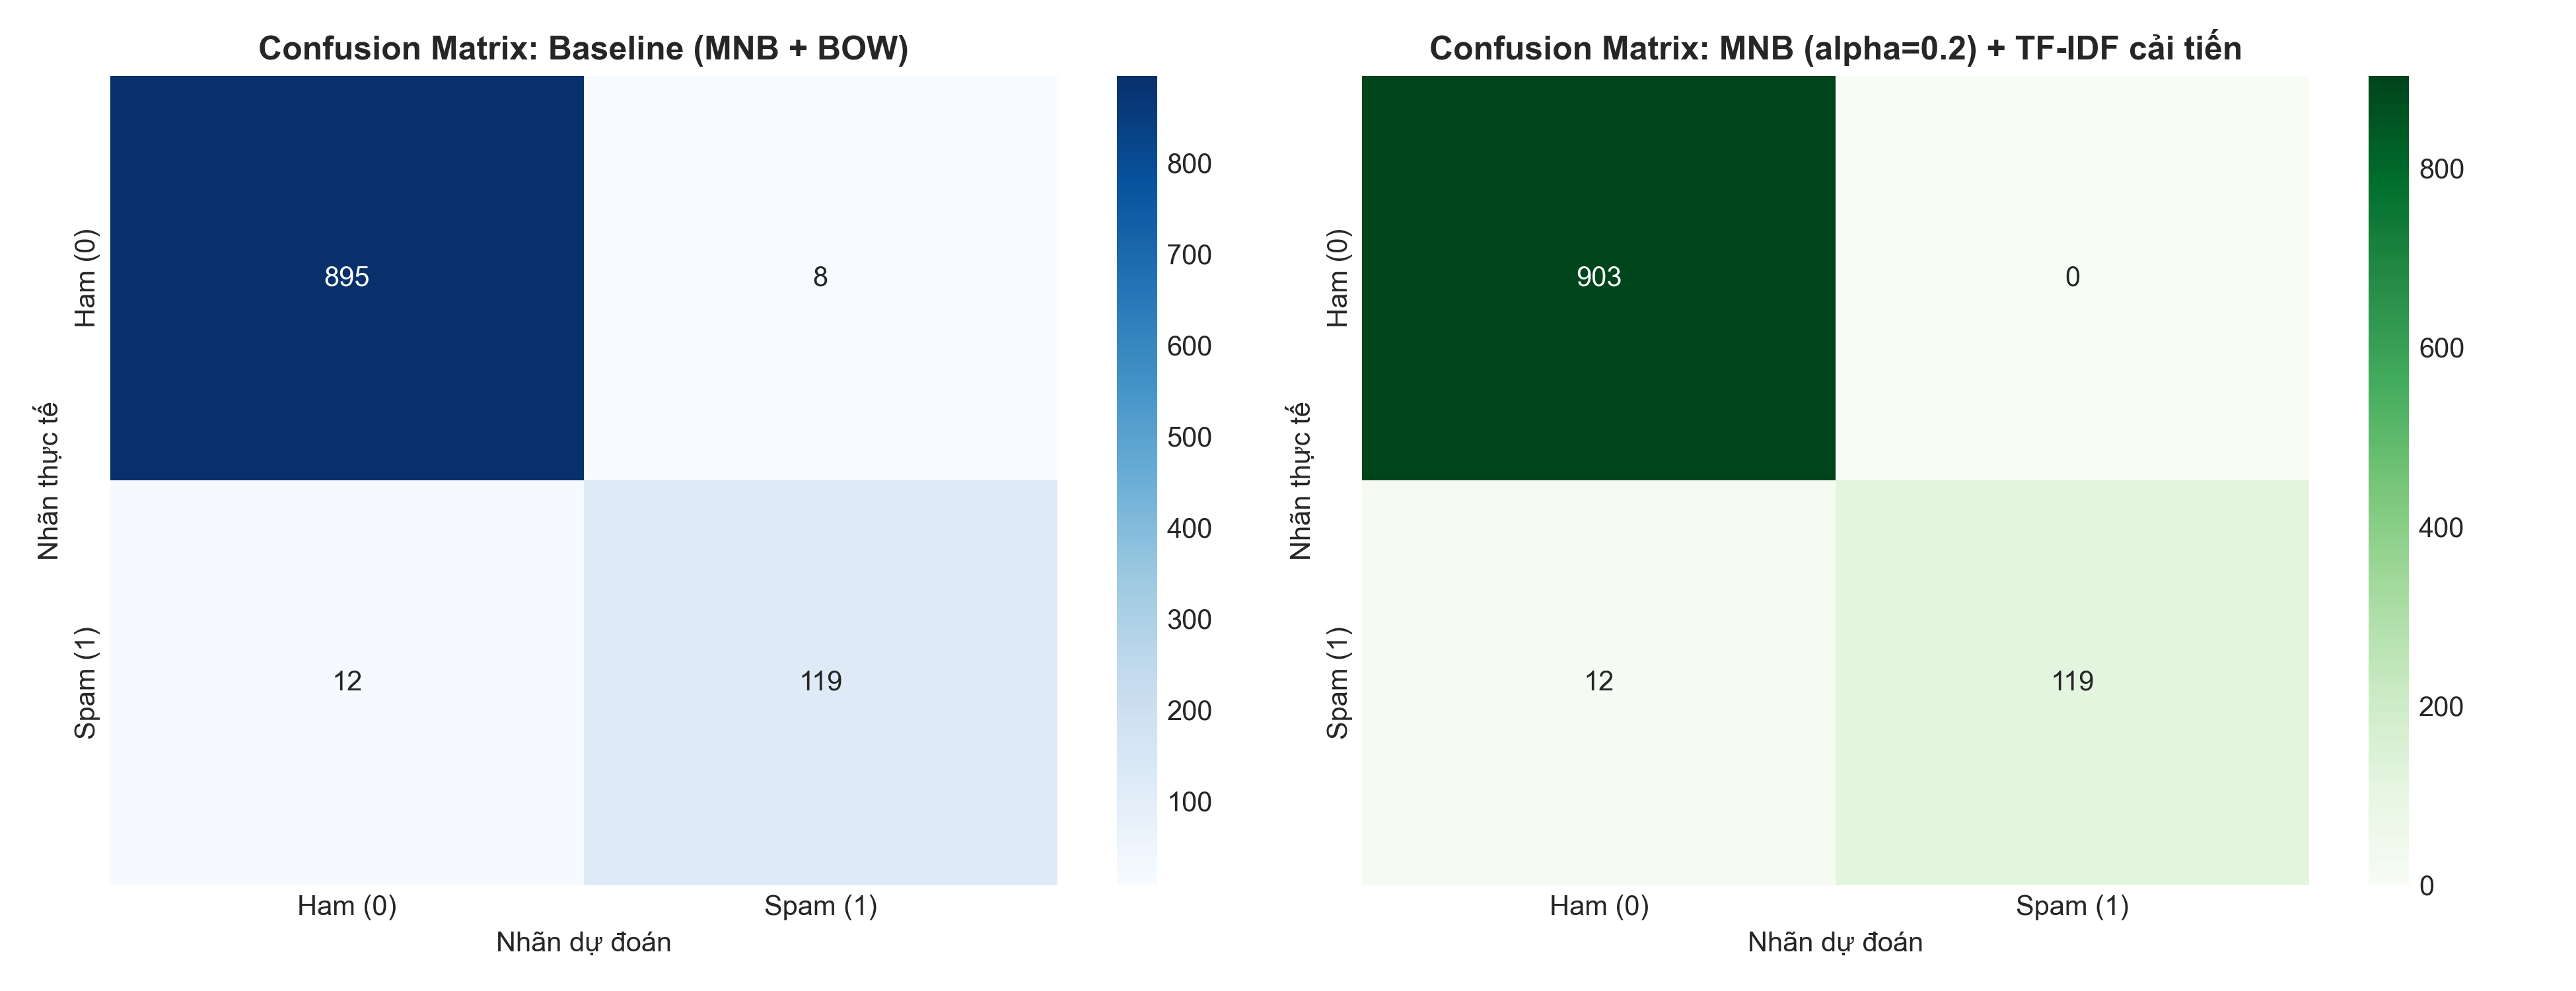
\includegraphics[width=0.95\textwidth]{figures/confusion_matrices.png}
    \caption{So sánh ma trận nhầm lẫn giữa Baseline (trái) và mô hình tối ưu MNB $\alpha=0.2$ + TF-IDF cải tiến (phải).}
    \label{fig:cm}
\end{figure}

Phân tích ma trận nhầm lẫn cho thấy một cải tiến mang tính quyết định về mặt nghiệp vụ: ở mô hình Baseline, có tới \textbf{8 tin nhắn hợp lệ (\texttt{ham})} bị phân loại nhầm thành \texttt{spam} ($FP = 8$). Khi chuyển sang Thí nghiệm 5, số lượng dương tính giả giảm xuống bằng \textbf{0} ($FP = 0$), đồng thời mô hình vẫn giữ nguyên khả năng bắt được $119 / 131$ tin nhắn rác thực tế ($TP = 119, FN = 12$). Điều này đồng nghĩa với việc hệ thống hoàn toàn không gây phiền toái hay làm thất lạc tin nhắn quan trọng của người dùng.

\subsection{Đánh giá tầm quan trọng của đặc trưng qua Log-odds Ratio}
Để lý giải cơ chế ra quyết định bên trong mô hình Multinomial Naive Bayes tối ưu, nhóm trích xuất chỉ số \textit{Log-odds ratio} cho từng đặc trưng $t_j$ trong bộ từ vựng 10.167 chiều:
\begin{equation}
    \text{Log-odds}(t_j) = \log P(t_j \mid y = \text{spam}) - \log P(t_j \mid y = \text{ham})
\end{equation}
Giá trị này càng lớn chứng tỏ sự xuất hiện của thuật ngữ $t_j$ làm tăng xác suất tin nhắn là \texttt{spam} càng mạnh. Biểu đồ Hình~\ref{fig:top_feat} hiển thị 15 đặc trưng có trọng số cao nhất.

\begin{figure}[H]
    \centering
    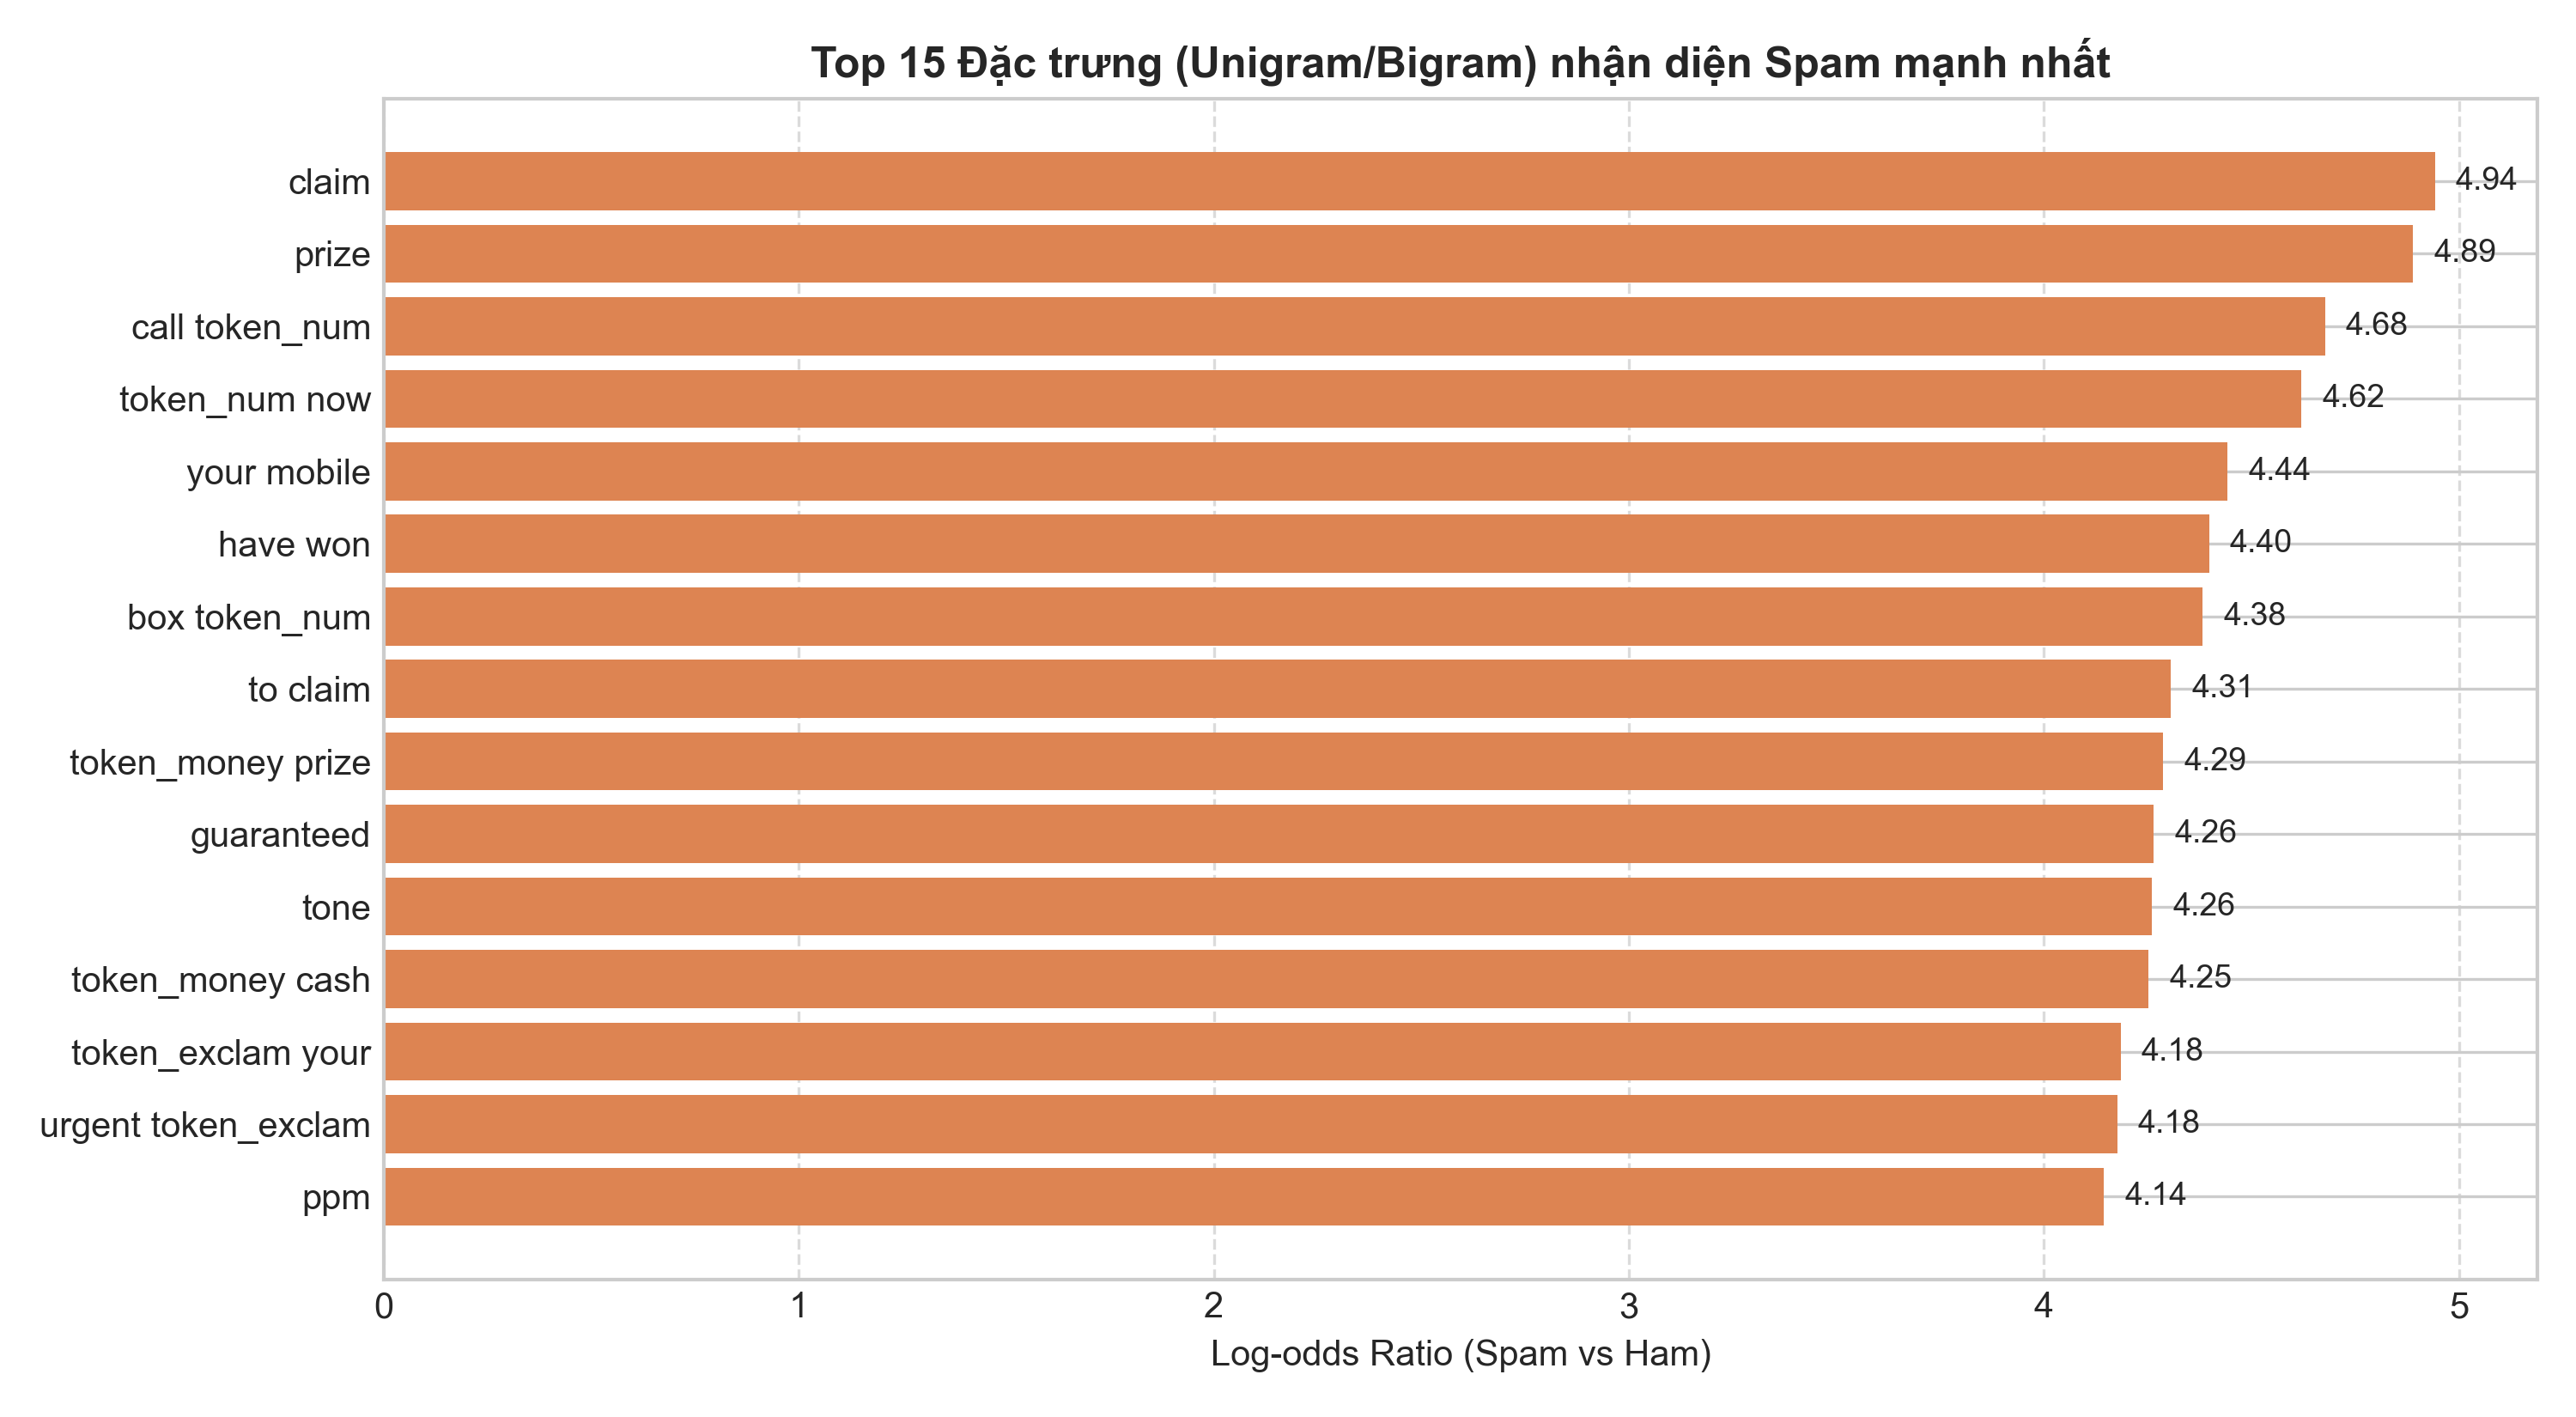
\includegraphics[width=0.92\textwidth]{figures/top_features.png}
    \caption{Top 15 đặc trưng (Unigram/Bigram) có trọng số Log-odds nhận diện tin nhắn rác cao nhất.}
    \label{fig:top_feat}
\end{figure}

Quan sát Hình~\ref{fig:top_feat} cho thấy bằng chứng thực nghiệm rõ ràng về hiệu quả của Phương án tiền xử lý 2: có tới \textbf{7 trong số 15 đặc trưng mạnh nhất} là các cụm từ bigram chứa các token ngữ nghĩa do nhóm tự thiết kế, bao gồm: \texttt{call token\_num} (4,68), \texttt{token\_num now} (4,62), \texttt{box token\_num} (4,38), \texttt{token\_money prize} (4,29), \texttt{token\_money cash} (4,25), \texttt{token\_exclam your} (4,18) và \texttt{urgent token\_exclam} (4,18). Việc gom nhóm các số điện thoại và giá trị tiền tệ cụ thể về các token chung đã giúp mô hình tổng quát hóa tốt các mẫu lừa đảo dù kẻ gửi thay đổi số điện thoại hay mệnh giá giải thưởng.

\section{Thảo luận chuyên sâu về thuật toán và siêu tham số}
\subsection{Tác động của hệ số làm mượt $\alpha$ trong Naive Bayes}
So sánh trực tiếp giữa Thí nghiệm 4 ($\alpha=1.0$) và Thí nghiệm 5 ($\alpha=0.2$) trên cùng ma trận đặc trưng TF-IDF cải tiến cho thấy một hiện tượng lý thuyết thú vị:
\begin{itemize}
    \item Khi giữ $\alpha=1.0$ (làm mượt Laplace tiêu chuẩn), \textit{Precision} đạt 100,00\% nhưng \textit{Recall} bị tụt xuống chỉ còn \textbf{79,39\%} (bỏ sót tới 27 tin nhắn rác). Nguyên nhân là do giá trị trọng số TF-IDF đã chuẩn hóa $L_2$ thường nằm trong khoảng nhỏ $(0, 1)$, trong khi mẫu số của ước lượng xác suất $N_c + \alpha |V|$ chịu ảnh hưởng lớn bởi kích thước từ vựng $|V| = 10.167$ và sự chênh lệch xác suất tiên nghiệm $P(\text{ham}) = 87,37\%$ so với $P(\text{spam}) = 12,63\%$. Hệ số $\alpha=1.0$ làm phẳng quá mức phân phối từ vựng của lớp thiểu số \texttt{spam}, khiến mô hình trở nên quá bảo thủ và có xu hướng thiên vị lớp đa số \texttt{ham}.
    \item Khi giảm hệ số làm mượt xuống $\alpha=0.2$ (làm mượt Lidstone), trọng số đóng góp của các từ khóa đặc trưng trong lớp \texttt{spam} được khôi phục đáng kể. Nhờ đó, \textit{Recall} tăng vọt thêm \textbf{+11,45\%} (lên mức 90,84\%) mà không làm phát sinh bất kỳ trường hợp bắt nhầm nào (\textit{Precision} vẫn giữ vững 100,00\%).
\end{itemize}

\subsection{Lý giải sự chênh lệch hiệu năng giữa MNB, Decision Tree và K-NN}
\begin{itemize}
    \item \textbf{Multinomial Naive Bayes} phù hợp nhất với bài toán phân loại văn bản ngắn vì thuật toán cộng dồn bằng chứng xác suất trên toàn bộ các từ xuất hiện trong câu. Ngay cả khi một tin nhắn thiếu vắng từ khóa phổ biến nhất (như \textit{``free''}), sự kết hợp của nhiều tín hiệu phụ (như \texttt{token\_num}, \texttt{urgent}, \texttt{claim}) vẫn đủ sức đẩy xác suất hậu nghiệm vượt qua ngưỡng phân loại.
    \item \textbf{Decision Tree} chỉ đạt $F_1 = 89,76\%$ và có thời gian huấn luyện chậm gấp 50 lần MNB (0,2064 giây) vì tại mỗi nút phân nhánh, cây chỉ kiểm tra sự xuất hiện của một từ khóa đơn lẻ. Với không gian 10.167 chiều và giới hạn độ sâu \texttt{max\_depth=20}, cây chỉ có thể bao phủ tối đa vài chục từ khóa chính, dẫn đến việc phân loại sai các tin nhắn rác sử dụng cách diễn đạt thay thế.
    \item \textbf{K-Nearest Neighbors} chỉ đạt $F_1 = 87,29\%$ do chịu tác động của hiện tượng \textit{lời nguyền số chiều} (Curse of Dimensionality). Tin nhắn SMS rất ngắn (trung bình chỉ khoảng 15--25 từ), khiến các vector trong không gian 10.167 chiều cực kỳ thưa thớt; khoảng cách cosine giữa một tin nhắn rác mới với 5 láng giềng gần nhất dễ bị nhiễu bởi các từ giao tiếp thông thường.
\end{itemize}

\section{Phân tích lỗi (Error Analysis) và hạn chế của hệ thống}
Nhằm đánh giá khách quan giới hạn của mô hình tối ưu (Thí nghiệm 5), nhóm trích xuất toàn bộ \textbf{12 mẫu tin nhắn rác bị bỏ sót} (False Negatives) trên tập kiểm thử và phân loại thành ba nhóm nguyên nhân cốt lõi như trình bày trong Bảng~\ref{tab:error_analysis}.

\begin{table}[H]
    \centering
    \caption{Phân loại nguyên nhân của 12 trường hợp âm tính giả (False Negatives) trên tập kiểm thử}
    \label{tab:error_analysis}
    \begin{tabular}{clp{6.5cm}}
        \toprule
        \textbf{Nhóm lỗi} & \textbf{Số lượng} & \textbf{Ví dụ trích xuất từ tập kiểm thử và phân tích nguyên nhân} \\
        \midrule
        1. Ngụy trang giao tiếp cá nhân & 5 mẫu & \textit{``Hi its LUCY Hubby at meetins all day wld u like to meet for a drink...''} --- Sử dụng đại từ thân mật (\textit{hi, hubby, babe, cool}), không chứa từ khóa khuyến mãi hay số điện thoại tổng đài nên giống hệt tin nhắn \texttt{ham}. \\
        2. Viết dính chữ / Ngoài từ điển & 4 mẫu & \textit{``Calls\pounds 1/minMobsmoreLKPOBOX177HP51FL''} --- Cố tình viết liền không khoảng trắng để né bộ tách từ, tạo ra các chuỗi ký tự lạ không đạt ngưỡng \texttt{min\_df=2} nên bị loại khỏi từ điển. \\
        3. Thông báo trung tính / Giải trí & 3 mẫu & \textit{``Missed call alert. These numbers called but left no message...''} --- Giả mạo thông báo hệ thống mạng di động với văn phong trung tính, thiếu các tín hiệu cảm xúc mạnh. \\
        \bottomrule
    \end{tabular}
\end{table}

\textbf{Hạn chế của giải pháp hiện tại:} Vì mô hình dựa trên biểu diễn túi từ (TF-IDF n-gram ở mức từ), hệ thống chưa nắm bắt được ngữ nghĩa sâu ở mức câu hoàn chỉnh và dễ bị tổn thương trước các kỹ thuật làm nhiễu văn bản cố ý (obfuscation) như viết dính liền nhiều từ hoặc thay thế chữ cái bằng ký tự tương tự.

% =========================================================================
% KẾT LUẬN VÀ HƯỚNG PHÁT TRIỂN
% =========================================================================
\chapter*{KẾT LUẬN VÀ HƯỚNG PHÁT TRIỂN}
\addcontentsline{toc}{chapter}{KẾT LUẬN VÀ HƯỚNG PHÁT TRIỂN}

\section*{1. Kết luận}
Bài tập lớn đã hoàn thành trọn vẹn các mục tiêu đề ra trong việc nghiên cứu, thiết kế và triển khai hệ thống phân loại tin nhắn rác tự động trên bộ dữ liệu chuẩn \textit{SMS Spam Collection v.1}. Những đóng góp và kết quả chính đạt được bao gồm:
\begin{enumerate}
    \item Thực hiện quy trình phân tích dữ liệu khám phá bài bản và thiết lập đường ống học máy chặt chẽ, loại bỏ 403 bản ghi trùng lặp và kiểm soát hoàn toàn hiện tượng rò rỉ dữ liệu giữa tập huấn luyện và tập kiểm thử.
    \item Đề xuất thành công phương pháp tiền xử lý chuyên biệt cho tin nhắn SMS bằng cách ánh xạ các thực thể quan trọng (\texttt{token\_url}, \texttt{token\_money}, \texttt{token\_num}, \texttt{token\_exclam}) kết hợp biểu diễn TF-IDF bigram, giúp nâng cao hiệu năng trên toàn bộ các thuật toán thử nghiệm.
    \item Tìm ra cấu hình tối ưu là \textbf{Multinomial Naive Bayes với hệ số làm mượt $\alpha = 0.2$}, đạt độ chính xác tổng thể \textbf{98,84\%}, \textbf{Precision đạt tuyệt đối 100,00\%} (không chặn nhầm bất kỳ tin nhắn hợp lệ nào) và \textbf{$F_1$-score đạt 95,20\%} (cải thiện $+2,95\%$ so với mô hình Baseline).
    \item Triển khai thành công ứng dụng web demo bằng thư viện Streamlit (\texttt{app.py}), cho phép kiểm thử mô hình trực quan theo thời gian thực.
\end{enumerate}

\section*{2. Hướng phát triển}
Để khắc phục các hạn chế đã chỉ ra trong phần phân tích lỗi và nâng cao khả năng ứng dụng thực tế, đề tài có thể mở rộng theo các hướng sau:
\begin{itemize}
    \item \textbf{Kết hợp đặc trưng mức ký tự (Character N-grams):} Bổ sung bộ trích xuất \texttt{analyzer='char\_wb'} với độ dài 3--5 ký tự để nhận diện hiệu quả các chuỗi từ cố tình viết dính liền hoặc biến thể chính tả.
    \item \textbf{Ứng dụng mô hình ngôn ngữ tiền huấn luyện (Pre-trained Language Models):} Thử nghiệm tinh chỉnh các kiến trúc Transformer gọn nhẹ như \textit{DistilBERT} hoặc \textit{TinyBERT} để nắm bắt ngữ cảnh sâu, giúp phát hiện các tin nhắn lừa đảo ngụy trang dưới dạng trò chuyện cá nhân.
    \item \textbf{Mở rộng sang ngữ liệu tiếng Việt:} Thu thập dữ liệu tin nhắn rác tiếng Việt và tích hợp bộ tách từ chuyên dụng (như \texttt{underthesea} hoặc \texttt{pyvi}) để triển khai hệ thống bảo vệ người dùng trong nước.
\end{itemize}

% =========================================================================
% TÀI LIỆU THAM KHẢO (Trình bày theo chuẩn APA)
% =========================================================================
\begin{thebibliography}{9}
\addcontentsline{toc}{chapter}{TÀI LIỆU THAM KHẢO}

\bibitem{almeida2011}
Almeida, T. A., Hidalgo, J. M. G., \& Yamakami, A. (2011). Contributions to the study of SMS spam filtering: New collection and results. In \textit{Proceedings of the 11th ACM Symposium on Document Engineering} (pp. 259--262). Association for Computing Machinery. \url{https://doi.org/10.1145/2034691.2034742}

\bibitem{bird2009}
Bird, S., Klein, E., \& Loper, E. (2009). \textit{Natural language processing with Python: Analyzing text with the natural language toolkit}. O'Reilly Media.

\bibitem{jurafsky2023}
Jurafsky, D., \& Martin, J. H. (2023). \textit{Speech and language processing} (3rd ed. draft). Stanford University. \url{https://web.stanford.edu/~jurafsky/slp3/}

\bibitem{manning2008}
Manning, C. D., Raghavan, P., \& Schütze, H. (2008). \textit{Introduction to information retrieval}. Cambridge University Press. \url{https://doi.org/10.1017/CBO9780511809071}

\bibitem{mccallum1998}
McCallum, A., \& Nigam, K. (1998). A comparison of event models for Naive Bayes text classification. In \textit{AAAI-98 Workshop on Learning for Text Categorization} (Vol. 752, No. 1, pp. 41--48). AAAI Press.

\bibitem{pedregosa2011}
Pedregosa, F., Varoquaux, G., Gramfort, A., Michel, V., Thirion, B., Grisel, O., Blondel, M., Prettenhofer, P., Weiss, R., Dubourg, V., Vanderplas, J., Passos, A., Cournapeau, D., Brucher, M., Perrot, M., \& Duchesnay, É. (2011). Scikit-learn: Machine learning in Python. \textit{Journal of Machine Learning Research}, 12(85), 2825--2830.

\bibitem{rennie2003}
Rennie, J. D., Shih, L., Teevan, J., \& Karger, D. R. (2003). Tackling the poor assumptions of Naive Bayes text classifiers. In \textit{Proceedings of the 20th International Conference on Machine Learning (ICML-03)} (pp. 616--623). AAAI Press.

\end{thebibliography}

% =========================================================================
% PHỤ LỤC: MÃ NGUỒN TRIỂN KHAI VÀ KHAI BÁO SỬ DỤNG AI
% =========================================================================
\appendix
\chapter{PHỤ LỤC MÃ NGUỒN HỆ THỐNG VÀ KHAI BÁO AI}

\section{Hàm tiền xử lý văn bản nâng cao và huấn luyện mô hình tối ưu}
Dưới đây là đoạn mã nguồn lõi thực hiện việc chuẩn hóa biểu thức chính quy thành các token ngữ nghĩa, vector hóa TF-IDF và huấn luyện mô hình Multinomial Naive Bayes tối ưu trong tệp \texttt{notebooks/01\_eda\_and\_modeling.ipynb}:

\begin{lstlisting}[language=Python, caption={Mã nguồn tiền xử lý nâng cao và huấn luyện mô hình tối ưu}]
import re
import joblib
import pandas as pd
from sklearn.model_selection import train_test_split
from sklearn.feature_extraction.text import TfidfVectorizer
from sklearn.naive_bayes import MultinomialNB
from sklearn.metrics import classification_report, accuracy_score

def clean_text_enhanced(text: str) -> str:
    """Chuan hoa van ban SMS thanh cac token ngu nghia chuyen biet."""
    text = text.lower()
    # 1. Chuan hoa dia chi URL
    text = re.sub(r'https?://\S+|www\.\S+', ' token_url ', text)
    # 2. Chuan hoa don vi tien te va gia tri tien
    text = re.sub(r'[\$\u00a3\u20ac]\s*\d+|\d+\s*(gbp|usd|vnd)', ' token_money ', text)
    # 3. Chuan hoa chuoi chu so (so dien thoai, ma thuong)
    text = re.sub(r'\b\d+\b|\d+', ' token_num ', text)
    # 4. Chuan hoa dau cham than cam xuc
    text = re.sub(r'!+', ' token_exclam ', text)
    # 5. Loai bo ky tu dac biet con lai, giu lai dau gach duoi cua token
    text = re.sub(r'[^a-z_\s]', ' ', text)
    text = re.sub(r'\s+', ' ', text).strip()
    return text

# Nap du lieu va khu trung lap truoc khi chia tap (chong Data Leakage)
df = pd.read_csv('data/SMSSpamCollection', sep='\t', names=['label', 'message'])
df = df.drop_duplicates().reset_index(drop=True)
df['target'] = df['label'].map({'ham': 0, 'spam': 1})
df['clean_enhanced'] = df['message'].apply(clean_text_enhanced)

X_train, X_test, y_train, y_test = train_test_split(
    df['clean_enhanced'], df['target'],
    test_size=0.2, stratify=df['target'], random_state=42
)

# Trich xuat dac trung TF-IDF (Unigram + Bigram)
tfidf_vec = TfidfVectorizer(ngram_range=(1, 2), min_df=2, max_df=0.95)
X_train_tfidf = tfidf_vec.fit_transform(X_train)
X_test_tfidf = tfidf_vec.transform(X_test)

# Huan luyen mo hinh Multinomial Naive Bayes tinh chinh (alpha=0.2)
best_mnb = MultinomialNB(alpha=0.2)
best_mnb.fit(X_train_tfidf, y_train)

y_pred = best_mnb.predict(X_test_tfidf)
print(f"Accuracy: {accuracy_score(y_test, y_pred):.4f}")
print(classification_report(y_test, y_pred, target_names=['Ham', 'Spam'], digits=4))

# Luu tru mo hinh de trien khai len ung dung Web
joblib.dump(tfidf_vec, 'models/tfidf_vectorizer.joblib')
joblib.dump(best_mnb, 'models/mnb_spam_classifier.joblib')
\end{lstlisting}

\section{Khai báo sử dụng công cụ Trí tuệ nhân tạo (AI)}
Tuân thủ quy định về liêm chính học thuật của Khoa Công nghệ Thông tin -- Trường Đại học Đại Nam, nhóm xin khai báo minh bạch việc sử dụng công cụ AI tạo sinh trong quá trình thực hiện bài tập lớn:
\begin{itemize}
    \item \textbf{Công cụ sử dụng:} Google Gemini.
    \item \textbf{Mục đích hỗ trợ:} Gợi ý cấu trúc tổ chức thư mục dự án khoa học dữ liệu, rà soát lỗi cú pháp thư viện giao diện Streamlit và hỗ trợ định dạng trình bày văn bản khoa học bằng hệ thống soạn thảo LaTeX.
    \item \textbf{Cam kết kiểm chứng và làm chủ sản phẩm:} Toàn bộ quy trình thu thập và khám phá dữ liệu, thiết kế biểu thức chính quy tiền xử lý, chạy thực nghiệm so sánh 7 kịch bản trên môi trường cục bộ, trích xuất biểu đồ và phân tích lỗi đều do sinh viên trực tiếp thực thi, kiểm tra tính đúng đắn của từng con số và sẵn sàng giải trình chi tiết trước hội đồng vấn đáp.
\end{itemize}

\end{document}